\subsection{Filter Design}

The typical Human can only hear frequencies in the range of 20Hz through 20kHz, and this range only decreases as humans age  \cite{human:rg}.  Using the website \url{http://onlinetonegenerator.com/hearingtest.html}, we will test the hearing range of each member listening to our final presentation.  This demonstration will provide a tangible example why appropriate filtering of an audio signal will have little to no impact on the quality of sound that a person hears after the filtering.  

When our project group performed the hearing test, the highest audible frequency was 15kHz.  Since our project group was not able to hear the frequencies above the 15kHz threshold, any low-pass filter that removed the high frequencies above 15kHz would have no impact on the quality of the audio signal that  we would hear.  Recall, removing the unecessary frequencies from an audio signal transmission provides a few nice benefits such as the following: 

\begin{enumerate}
\item It reduces the necessary power for transmission of the audio signal
\item It reduces the necessary bandwidth for transmission
\end{enumerate}

Filtering is the processing of a time-domain signal resulting in some change in that signals original spectral content.  The change is usually the reduction or filtering of unwanted input spectral components.\cite{lyons:intro}.  Given the human threshold for hearing, an obvious opportunity is to apply low-pass filtering in order to transmit audio signals that humans can actually hear with smaller bandwidths.  The ideal low pass filter would completely eliminate all frequencies above a certain cutoff point (in our hearing test example, the cutoff would be at 15kHz) while passing all frequencies below the cutoff point \cite{lowpass:wiki}.       

\begin{figure}[h!]
	\centering
	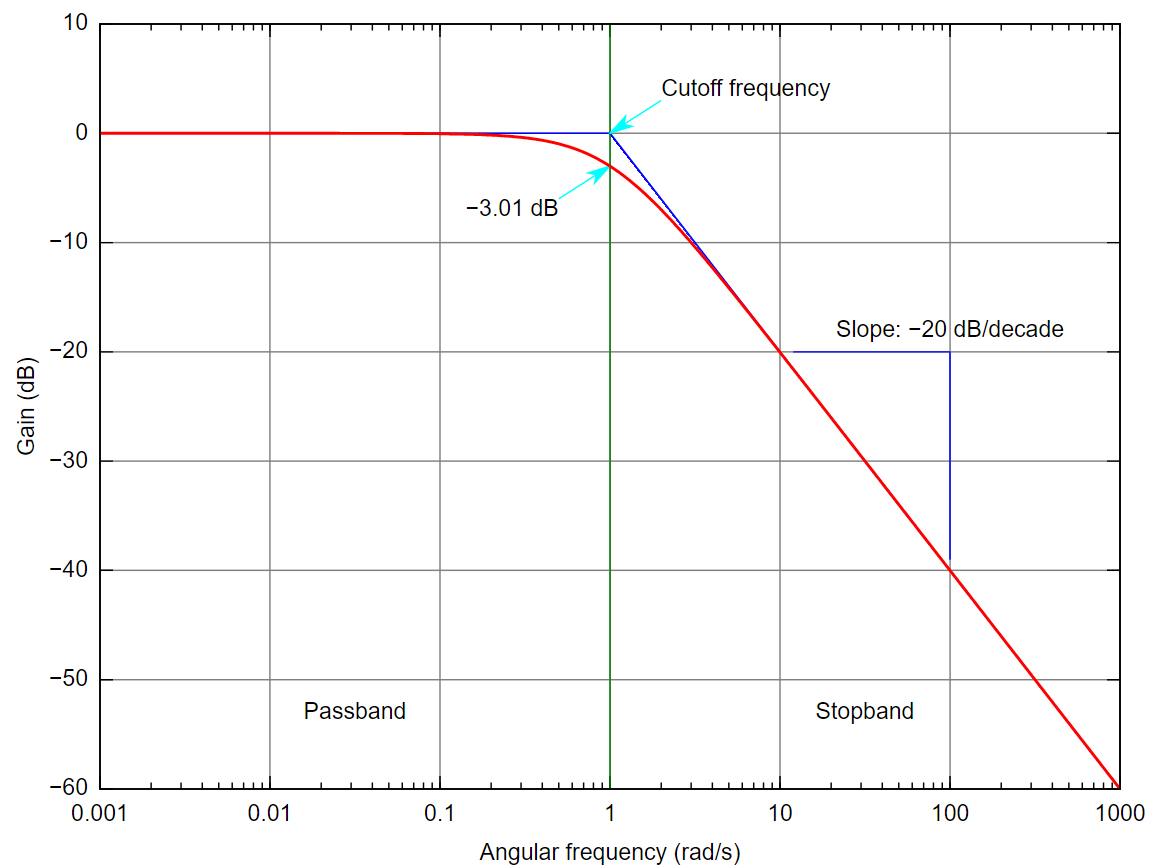
\includegraphics[scale = .5]{low_pass.png} %this is useful too \includegraphics[width = \linewidth]
	\caption{Example of Low Pass Filter: \url{https://upload.wikimedia.org/wikipedia/commons/6/60/Butterworth_response.svg}}
	\label{fig:lowpass}
\end{figure}    

In order to filter out higher frequencies in an audio signal transmission, we will build a low pass filter.  Specifically, we will describe how a low pass filter is created using a finite number of non-zero filter coefficients which is called a \textit{Finite Impulse Response} filter or FIR.  Given an impulse response, we can find the coefficients of the filter, and vice versa \cite{notes:class}.  For example, Figure \ref{fig:lowpass} shows a graphical depiction of a low pass filter that begins to cut out the frequencies above 1 rad/s.  Frequencies below the cutoff frequency are considered to be in the ``Passband," or allowable frequency band.  Frequencies above the cutoff frequency filtered out and are considered in the ``Stopband."  Ideally, the slope between the Passband and the Stopband would be as steep as possible to limit the passing of unwanted high audio frequencies.  The question still remains, how do you build a filter that eliminates these frequencies?  What is an impulse response?  Why do we need to find coefficients of a filter and what do they do?  Let's address those questions next. 

\subsubsection{Impulse Input, Impulse Response, and FFT}

	In our filtering example, we will be dealing with a Linear Time-Invariant (LTI) System.  A linear system is a class of systems where the system's outputs are the sum of the outputs of it's parts.  Additionally, Time-Invariant refers to a system where a time delay in the input sequence causes an equivalent delay in the output sequence.  Now, if we are given a LTI system, we can calculate everything about the system if we know the \textit{unit impulse response}.  The \textit{unit impulse response} refers to the system's time-domain output sequence when the input is a single unity-valued sample (unit impulse) surounded by zero-valued samples.  Furthermore, knowing the impulse response of an LTI system, the \textit{output sequence} is calculated by taking the \textit{convolution}  of the input sequence and the system's impulse response \cite{lyons:intro}.  We will talk more about convolutions later, but we typically do not perform convolutions in the time domain since they are computationally expensive.  Instead, multiplication is performed in the frequency domain.  In order to transform the impuse response into a \textit{frequency response}, we take the Fast Fourier Transform (FFT) of the impulse response\cite{lyons:intro}.

Let's explain with a simple example, if we let $x(n)$ be a discrete-time sequence of individual signal amplitudes, then we can define a simple LTI \textit{averager} system as follows: 

$$y(n) = \frac{1}{4} \left[ x(n)+x(n-1)+x(n-2)+x(n-3)\right] =  \frac{1}{4}\sum_{k=n-3}^{n} x(k)$$    

Given, this simple averager, we can show the block diagram in Figure \ref{fig:impulse} (a), impulse input and impulse response in Figure \ref{fig:impulse} (b), and the frequency magnitude response created from the FFT of the impulse response in Figure \ref{fig:impulse} (c).  The block diagram in Figure \ref{fig:impulse} (a) - also referred to as the \textit{Filter Structure}, simply shows how an impulse input is transformed into a impulse response.  The impulse response, $y(n)$, is created by passing the impulse input, $x(n)$, into the system and storing the four most recent values.  Once there are four values, they are added together and multiplied by $\frac{1}{4}$ to calculate the average.  The sequence proceeds one step averaging the most recent four values of the impulse input, $x(n)$, along the way.  Since there are four separate input sample values to calculate an output value, the structure of this filter can be referred to as a \textit{4-tap tapped-delay line FIR filter} using digital filter vernacular.  The coefficients of this filter are all $\frac{1}{4}$ and we can use an Fast Fourier Transform on the filter to provide all the frequency domain information.

\begin{figure}[h!]
	\centering
	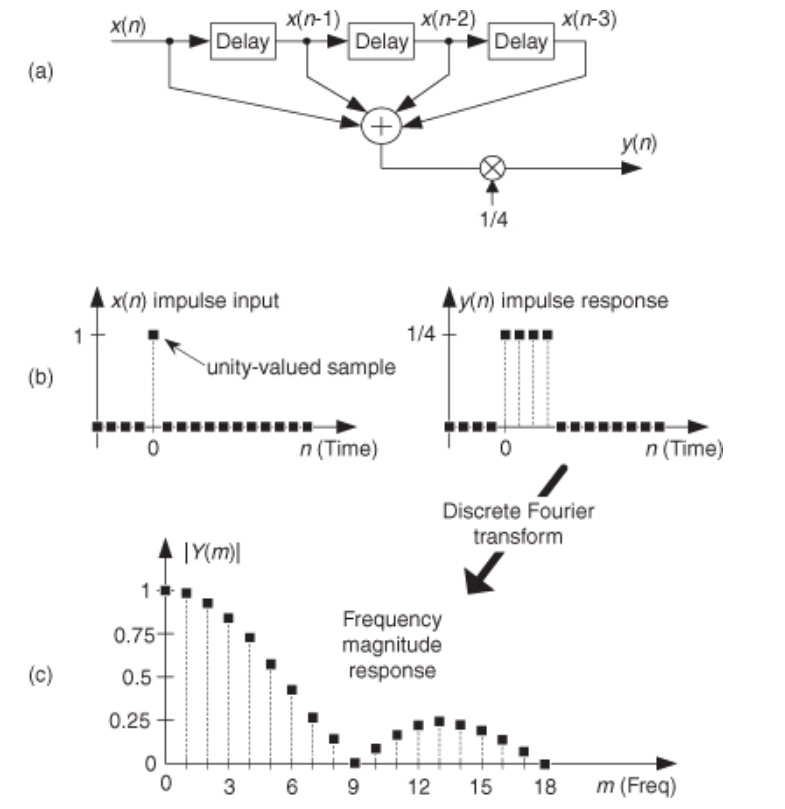
\includegraphics[scale = .6]{impulse.png} %this is useful too \includegraphics[width = \linewidth]
	\caption{Block Diagram (a), Impulse Input and Impulse Response (b), and Frequency Magnitude Response after FFT of Impulse Response (c).  Taken from Reference \cite{lyons:intro} below and is Figure 1-12 from Chapter 1}
	\label{fig:impulse}
\end{figure}    

From Figure \ref{fig:impulse} (c), the FFT transforms the impulse response $y(n)$ into $Y(m)$, which is the frequency domain information.  $Y(m)$ provides the frequency magnitude response of the simple 4-point averager.  This is actually an example of a low pass filter where the \textit{averager} reduces the amplitude (attenuates) the high-frequency  signal.  In our construction of a filter, we will have to use a different impulse response since we want to remove, not attenuate, the high frequency information content.  The following section will explain how we design a Finite Impulse Response (FIR) filter using the window method in order to create a low pass filter that removes high frequency information content. 

\subsubsection{Finite Impulse Response (FIR)}

An FIR filter has a finite duation of nonzero output values given a finite duration of input values (this is how they were named!).  Recall, in our example above, we used four ``taps" that were all equal to $\frac{1}{4}$.  The two factors that affect an FIR filter's frequency response are the number of taps and the coefficients\cite{lyons:intro}.  If we were to calculate the impulse response, $y(n)$, from the impulse input, $x(n)$, in the time-domain, then we would have to perform the mathematical operation of a convolution.  More specifically for an \textit{M}-tap filter, we would calculate $y(n)$ as follows: 

$$y(n) = \sum_{k=0}^{M-1}  h(k)x(n-k)$$

Where $h(k)$ are the filter coefficients for each of the taps.  \textbf{The terms FIR filter coefficients and impulse response mean the same thing}\cite{lyons:intro}.  We can re-write the above equation using \textit{convolution} notation as follows: 

$$y(n) = h(k) \star x(n)$$  

The major concept is that convolution in the time domain is equal to multiplication in the frequency.  The process in which we can move from one domain to the other is through the Fast Fourier Transform (FFT).  The FFT of $y(n)$ is equal to $Y(m) = H(m) X(m)$, which is the spectrum of the filter output.  In a similar way, we can determine $h(k)\star x(n)$ by taking the inverse of the FFT (we will denote this as IDFT - Inverse Discrete Fourier Transform)\cite{lyons:intro}.  The important relationships are as follows: 

\begin{enumerate}
\item $x(n) \overset{FFT}{\longrightarrow} X(m)$
\item $X(m) \overset{IDFT}{\longrightarrow} x(n)$
\item $h(k) \overset{FFT}{\longrightarrow} H(m)$
\item $H(m) \overset{IDFT}{\longrightarrow} h(k)$
\item $y(n) \overset{FFT}{\longrightarrow} Y(m) \Rightarrow h(k)\star x(n) \overset{FFT}{\longrightarrow} H(m) X(m)$
\item $Y(m) \overset{IDFT}{\longrightarrow} y(n) \Rightarrow H(m) X(m) \overset{IDFT}{\longrightarrow} h(k)\star x(n)$
\end{enumerate}    

Now that we can easily move between the frequency and time-domains using the FFT or IDFT, let's design our own low-pass filter by determining the desired frequency response and moving back to the time domain through an IDFT to calculate the filter coefficients that will provide the desired frequency response.  Recall, in our hearing test example, our project group was unable to hear any frequency information content above 15kHz.  As such, we will attempt to design a low-pass filter that removes all of the frequency content above this threshold.  Therefore, our \textit{cutoff} frequency is 15kHz (see Figure \ref{fig:lowpass} for a depiction of the cutoff frequency).  The method that we will use is to define the individual frequency-domain samples representing $H(m)$, and then use Python and the inverse FFT function on these samples to give the FIR filter coefficients.  In order to do this, we must define $H(m)$ over the frequency span from 0 to $f_s$, where $f_s$ is the sampling rate.  As we will discuss in the next section, the sampling rate that we will use is $f_s = 44.1$ kHz.         
  
 
